\documentclass[a4paper,oneside]{article}

\usepackage{graphicx}

\begin{document}

Figure \ref{fig:dbs} shows the database schema. I have introduced the Member table in the schema
as well, although not required, in order to be able to show how the MGMembers table links to it.
Clearly, the only thing that should conform to this design in what the real Member table is
concerned, is the existence of the \emph{id} field. All the other fields are irrelevant.
\\
\begin{figure}[ht]
	\centering
	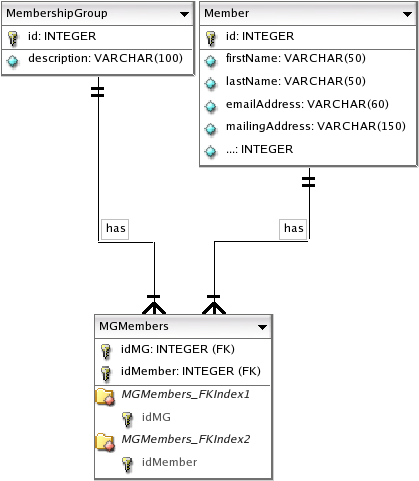
\includegraphics[bb=0 0 165 189]{db-schema.png}
% db-schema.png: 72.009dpi, width=5.82cm, height=6.67cm, bb=0 0 165 189
	\caption{The database schema}
	\label{fig:dbs}
\end{figure}

Figure \ref{fig:os} shows the object schema. Again, the Member class appears only for reference
purposes. The relationship between the two classes indicates that a MembershipGroup has zero or
more Members, while a Member belongs to zero or more MembershipGroups. In order to be able to
properly simulate the functionality, I will, however, have to create the Member class and implement
the methods shown in the diagram.
\\
\begin{figure}[ht]
	\centering
	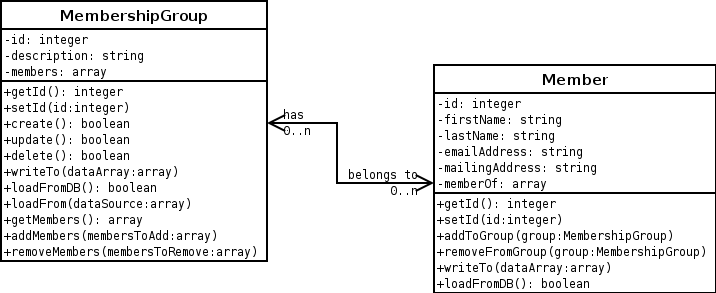
\includegraphics[bb=0 0 282 103]{obj-schema.png}
% obj-schema.png: 50.8dpi, width=14.10cm, height=5.15cm, bb=0 0 282 103
	\caption{The object schema}
	\label{fig:os}
\end{figure}

\end{document}